\documentclass[9pt]{beamer}
\geometry{paperwidth=140mm,paperheight=105mm}
\usepackage[utf8]{inputenc}
\usepackage{amsmath}
\usepackage{amsfonts}
\usepackage{amssymb}
\usepackage[cal=boondox-cal]{mathalfa}
\usepackage{soul}
\usepackage{ulem}
\usepackage{fancyvrb}
\usepackage{calrsfs}
\usepackage{float}
\usepackage{xcolor}

\usepackage[scr=boondoxo,scrscaled=1.05]{mathalfa}


\usetheme{Frankfurt}
% Slide numbering
\addtobeamertemplate{navigation symbols}{}{%
    \usebeamerfont{footline}%
    \usebeamercolor[fg]{footline}%
    \hspace{1em}%
    \insertframenumber/\inserttotalframenumber
}
\setbeamercolor{footline}{fg=blue}
% Work block config (green blocks)
\newenvironment{workblock}[1]{%
  \setbeamercolor{block body}{bg=green!10}
\begin{block}{#1}}{\end{block}}
\setbeamerfont{workblock body}{size=\tiny}

%Information to be included in the title page:
% logo
\titlegraphic{
    
\includegraphics[width=1.5cm]{figures/ENSG_logo.png}\hspace*{9cm}~%
    
\includegraphics[width=1.3cm]{figures/IPGP_logo.png}
}
\title[\normalsize Un titre raccourci pour l'affichage en bas de slide]{Titre du stage à rallonge}
\author[Prénom Nom]{Prénom \textsc{Nom}\\
    \emph{Maître de Stage :} Prénom \textsc{Nom}\\
    \emph{Professeur référent :} Prénom \textsc{Nom}\\}
\date{\normalsize Date}


\begin{document}

\frame{\titlepage}


\section*{Introduction}

\begin{frame}
\frametitle{Introduction : sources de déformation de la Terre}
    \centering
    \includegraphics[height=0.80\textheight]{figures/schéma_charges.png}
    
\end{frame}

\begin{frame}
\frametitle{Introduction : déformation de la Terre observée}
    \centering
    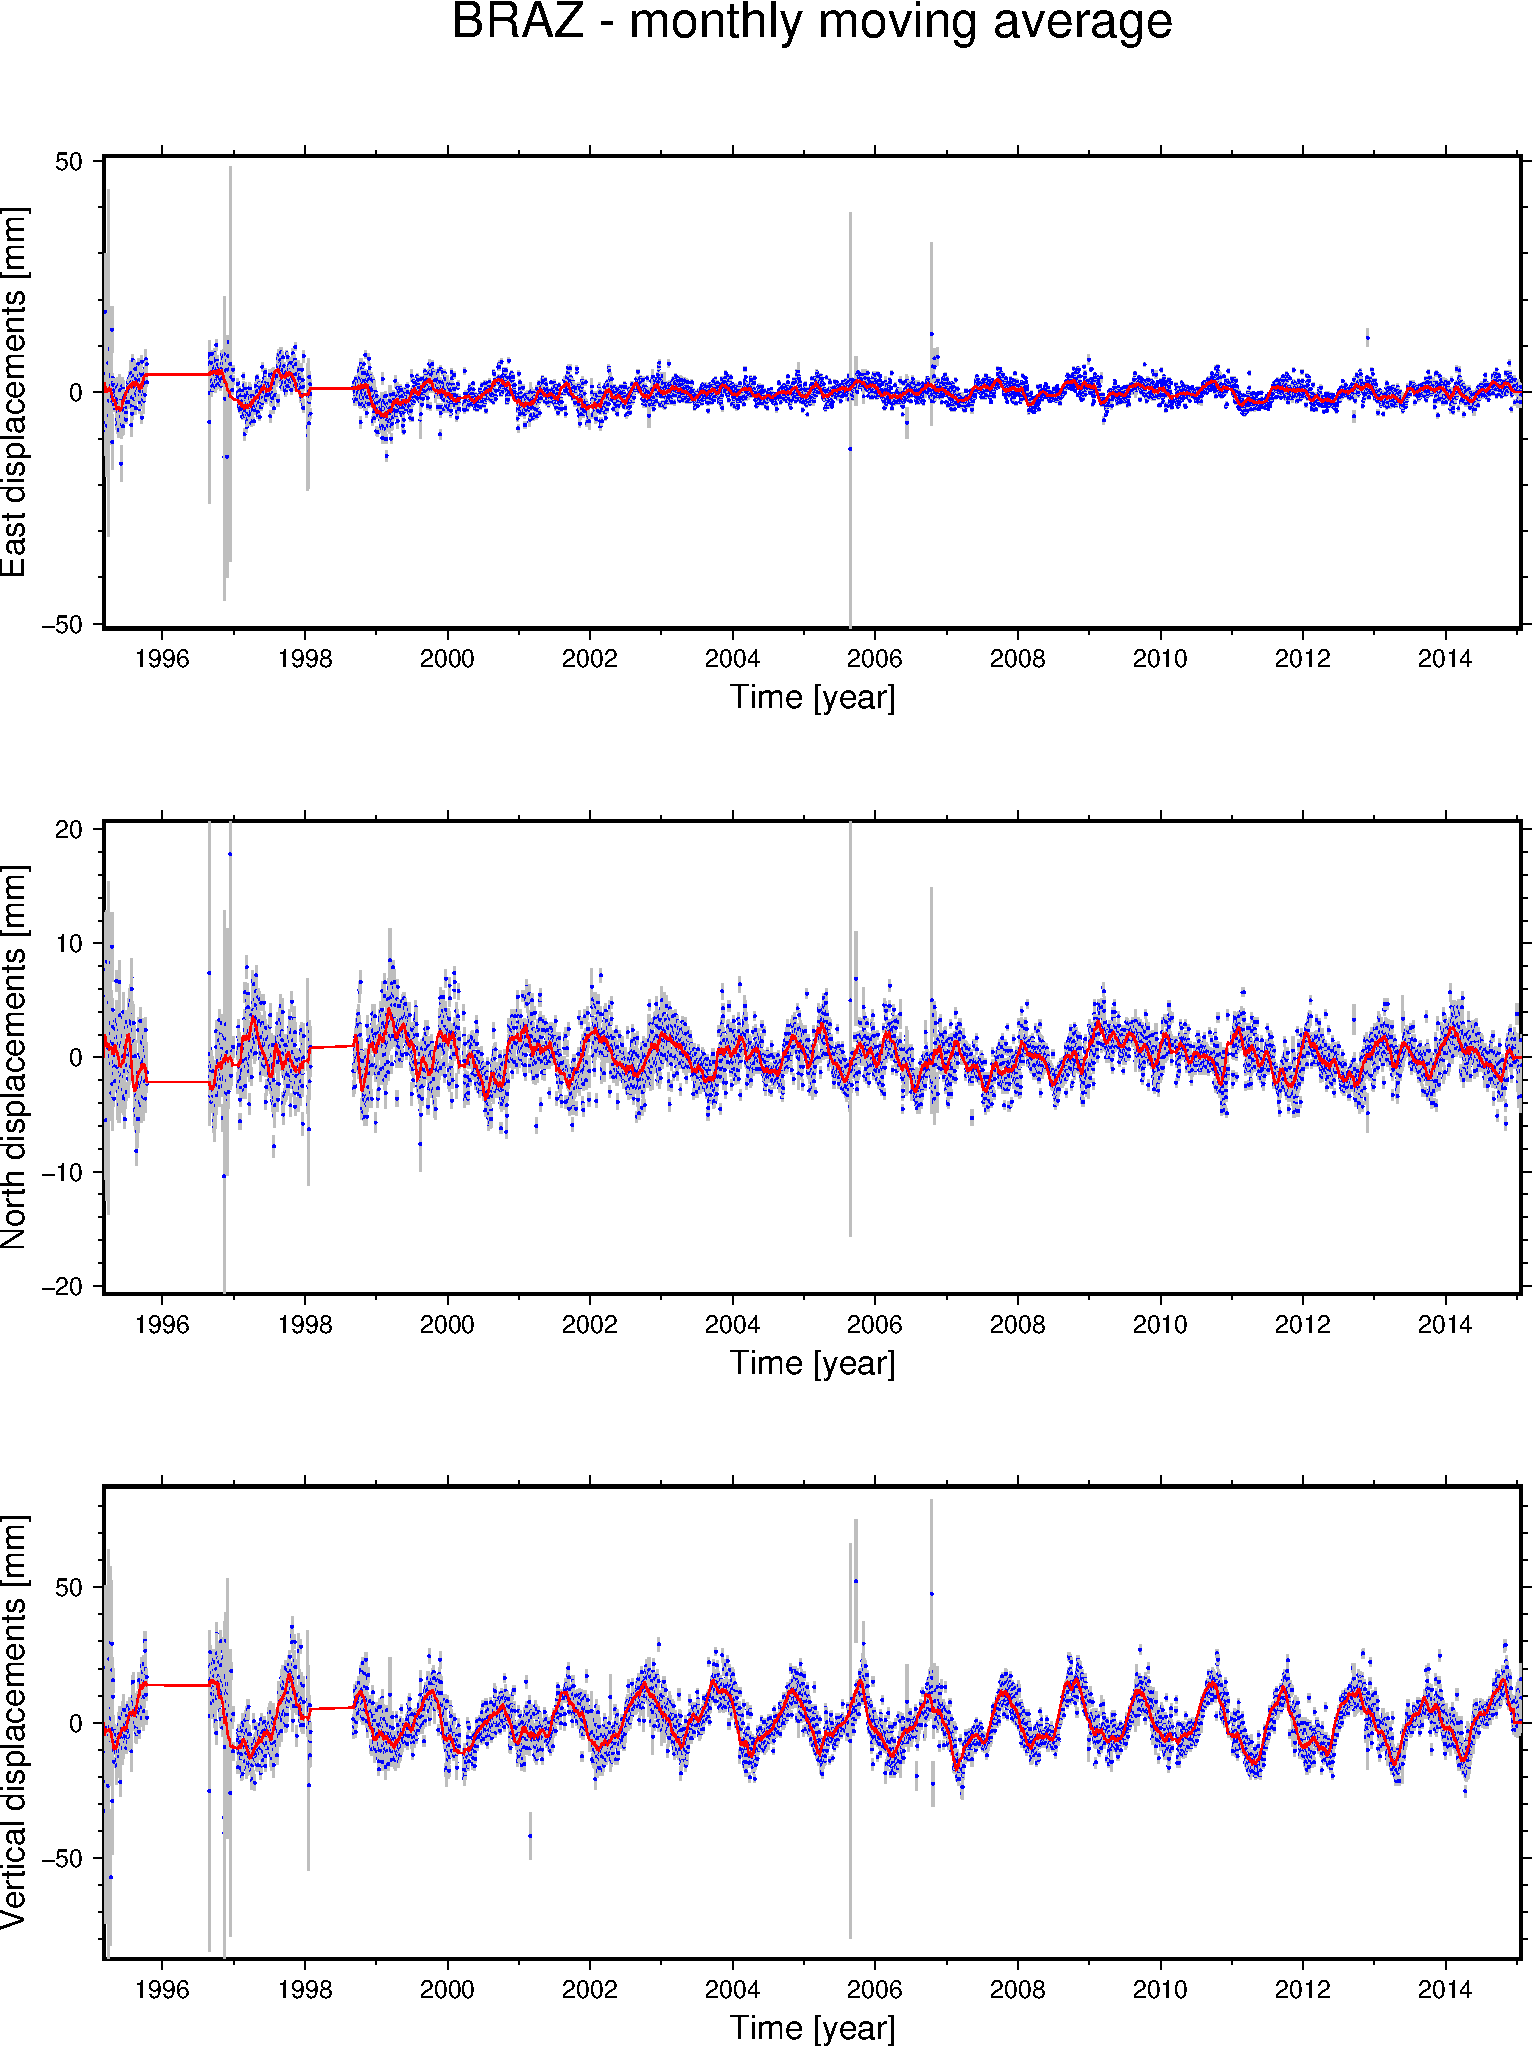
\includegraphics[width=0.40\textwidth]{figures/BRAZ_ma.pdf}
    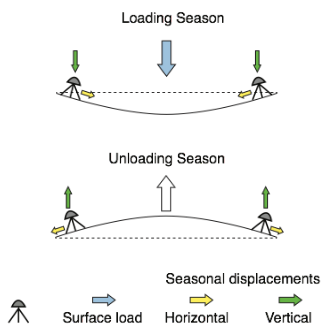
\includegraphics[ width=0.40\textwidth]{figures/schema_gps_load_vertical.png}
        \begin{block}{Question scientifique}
    Dans quelle mesure les modèles de charge expliquent-ils les déplacements mesurés par GNSS ?
    \end{block}
    $\rightarrow$ Jiang et al. (2013) \\ $\rightarrow$ Li et al. (2016)
\end{frame}



\begin{frame}
\frametitle{Plan}
\tableofcontents
\end{frame}


\section{Données}

\begin{frame}
    \frametitle{Données GNSS}
    \begin{columns}
        \begin{column}{0.5\textwidth}
        \centering
            International GNSS Service (IGS), 
            2nd Data Reprocessing Campaign\\
            \vspace{0.2cm}
            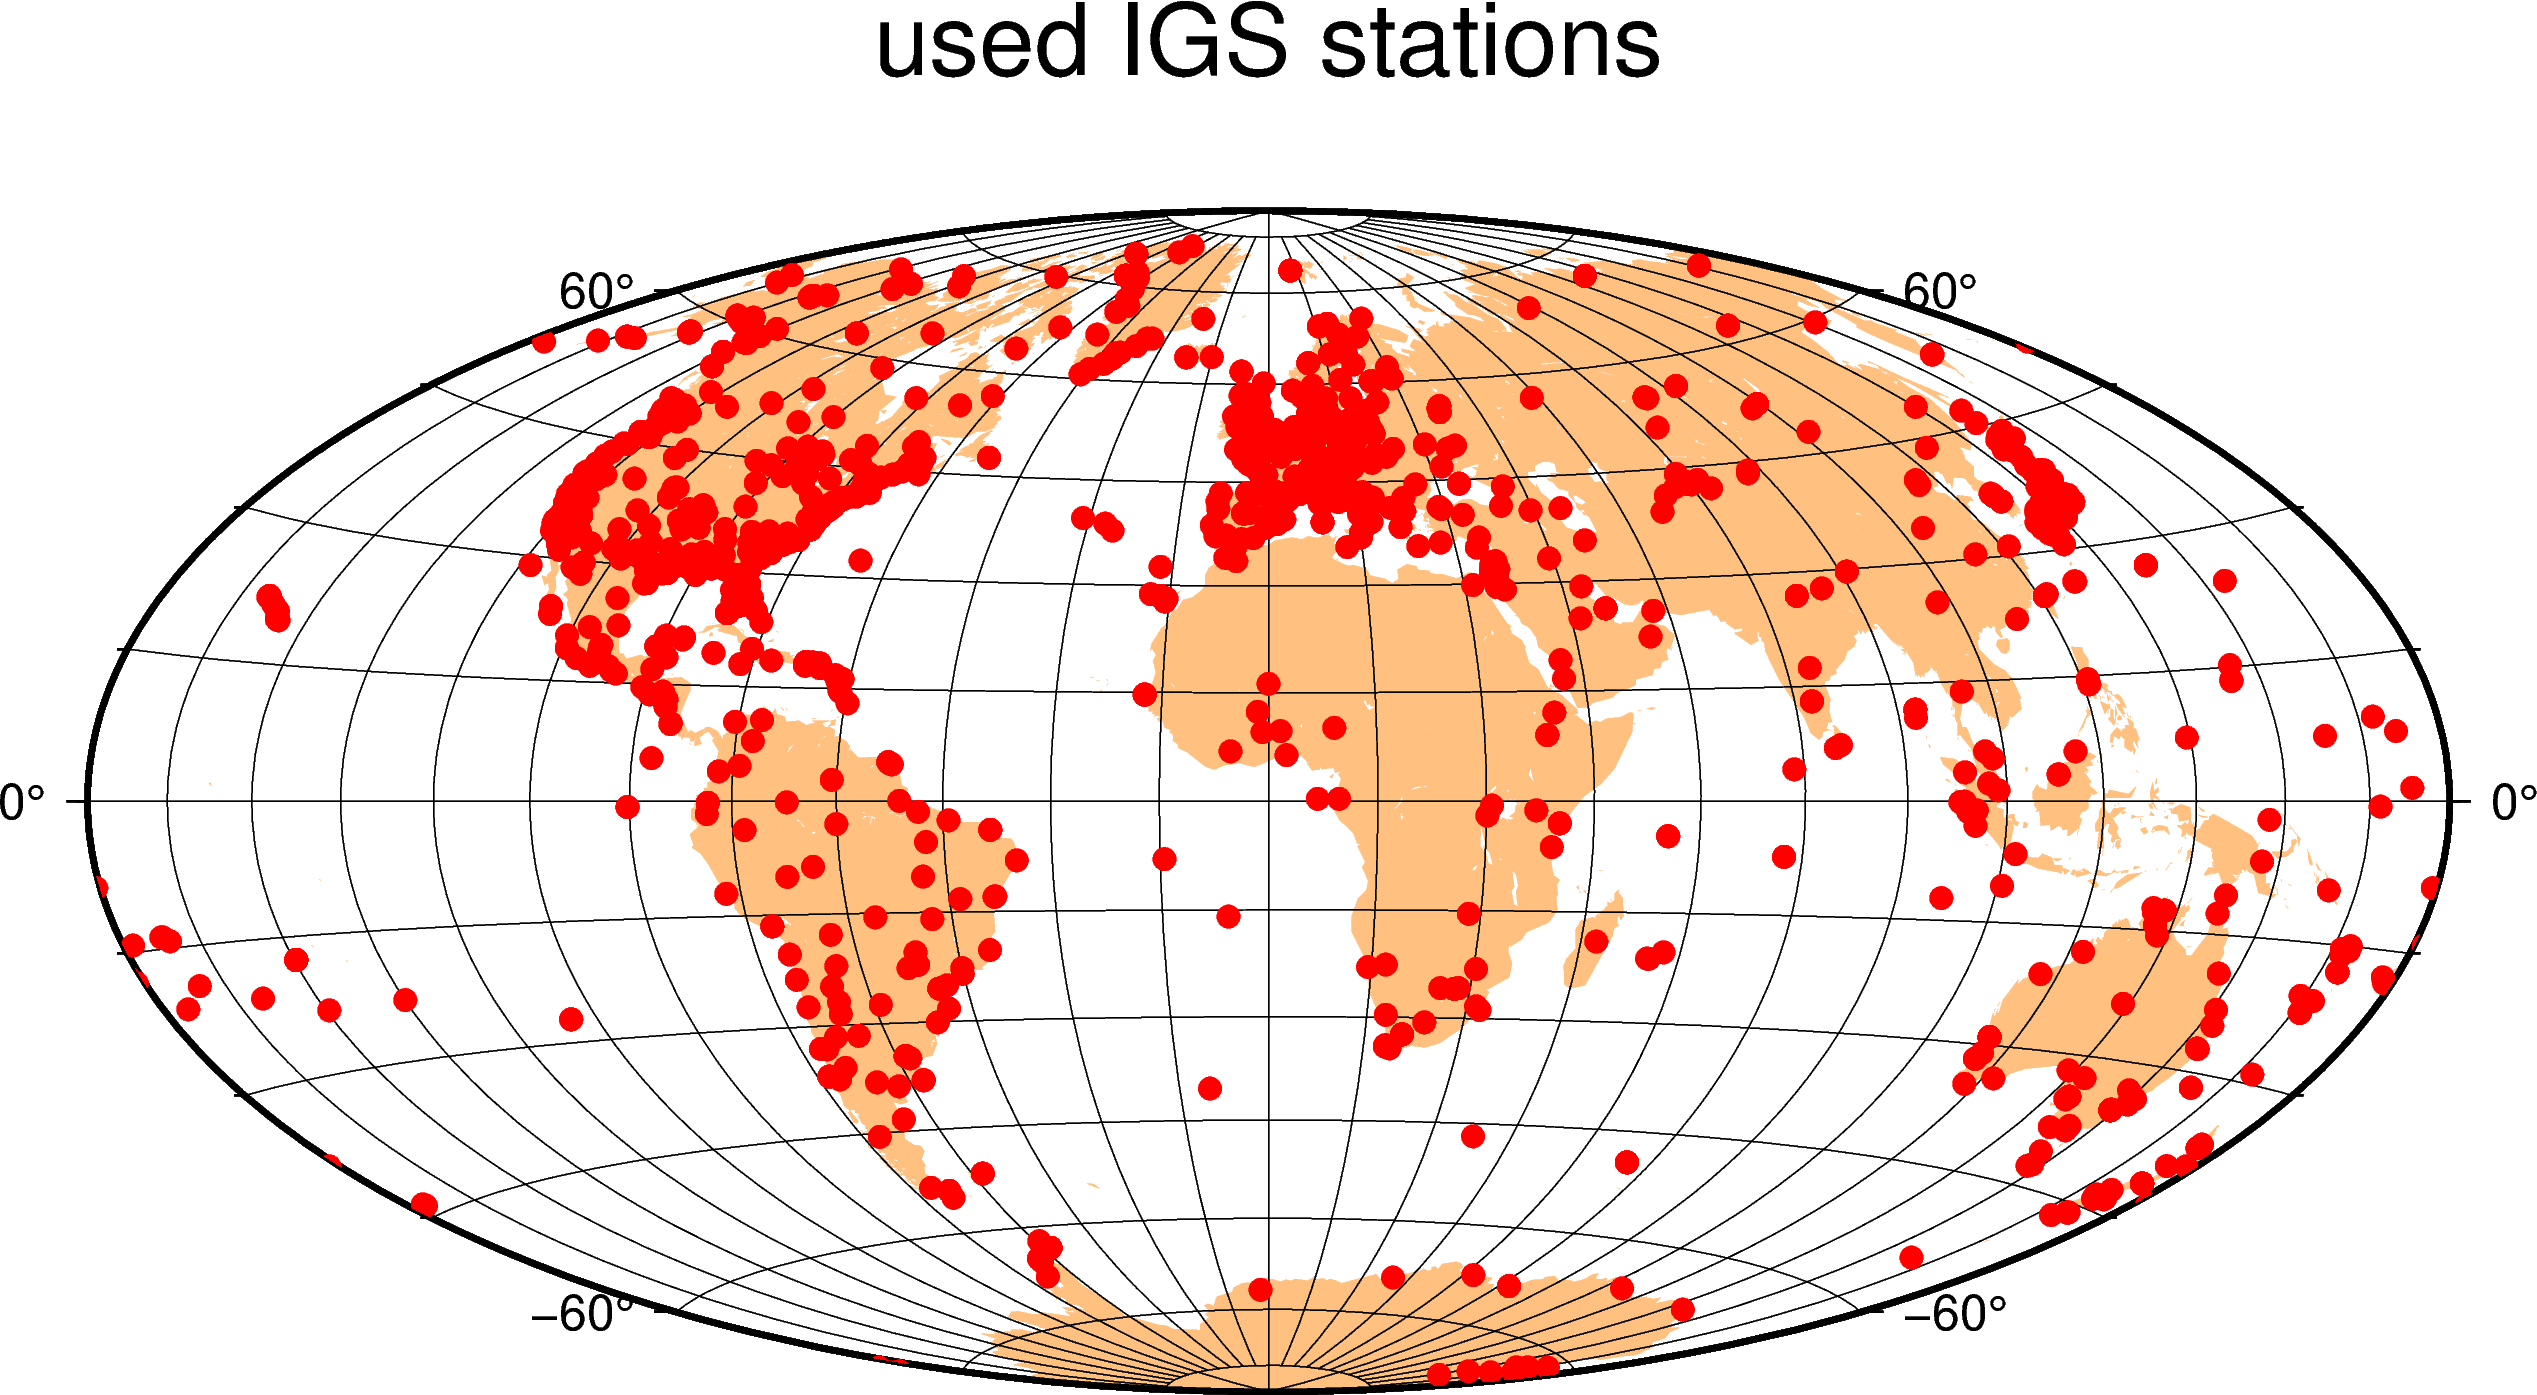
\includegraphics[width=\textwidth]{figures/sd_ig2.png}
            \hyperlink{http://acc.igs.org/reprocess2.html}{ \verb #http://acc.igs.org/reprocess2.html# }\\
        \end{column}
        \begin{column}{0.5\textwidth}
            \centering
            Nevada Geodetic Laboratory (NGL)\\
            \vspace{0.5cm}
            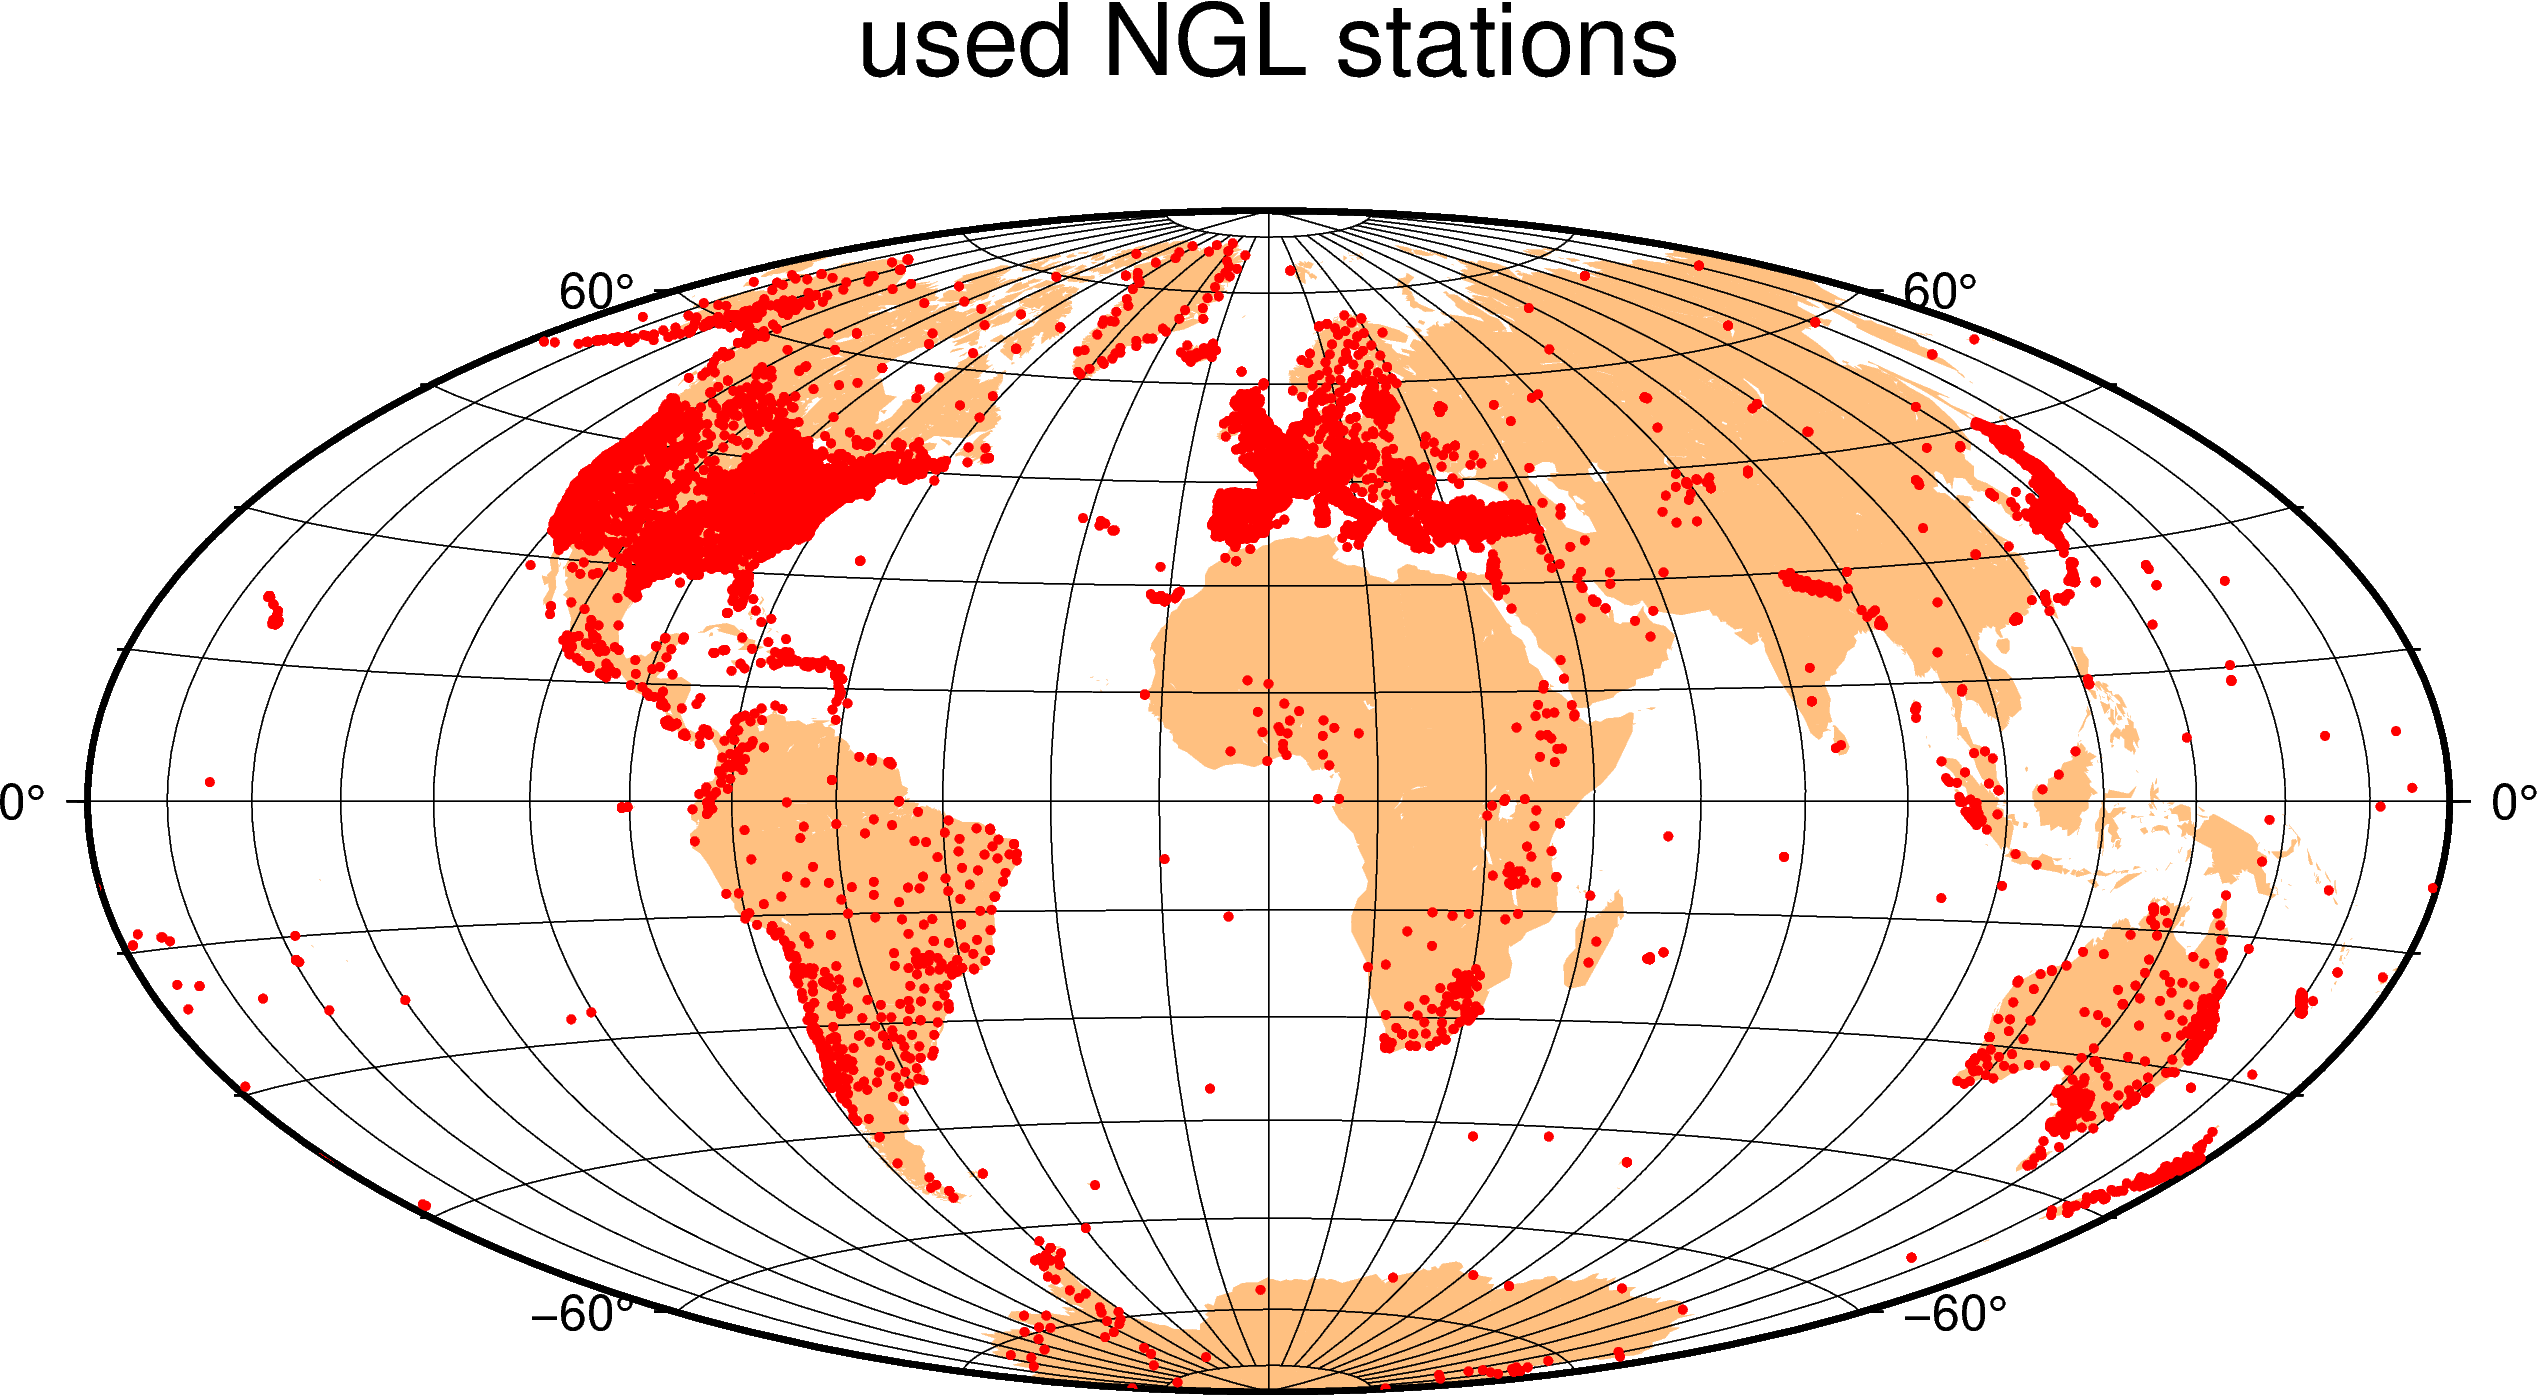
\includegraphics[width=\textwidth]{figures/sd_ngl.png}
            \hyperlink{http://geodesy.unr.edu/gps/ngl.acn.txt}{ \verb #http://geodesy.unr.edu/gps/ngl.acn.txt# }\\ 
        \end{column}
    \end{columns}
    \vspace{0.5cm}
    Données corrigées :
    \begin{itemize}
        \item  des sauts : co-sismique, changement de matériel
        \item des déplacements locaux de plaques tectoniques
        \item de la déformation post-sismique
    \end{itemize}
    
     \begin{workblock}{}
     \small{Développement d'un module Python pour le post-traitement des données.\\ Apprentissage de GMT et pyGMT pour le tracé de cartes et graphes.}
     \end{workblock}
\end{frame}

\begin{frame}
\frametitle{Gravity Recovery And Climate Experiment (GRACE)}

\begin{columns}
        \begin{column}{0.2\textwidth}
        \centering
          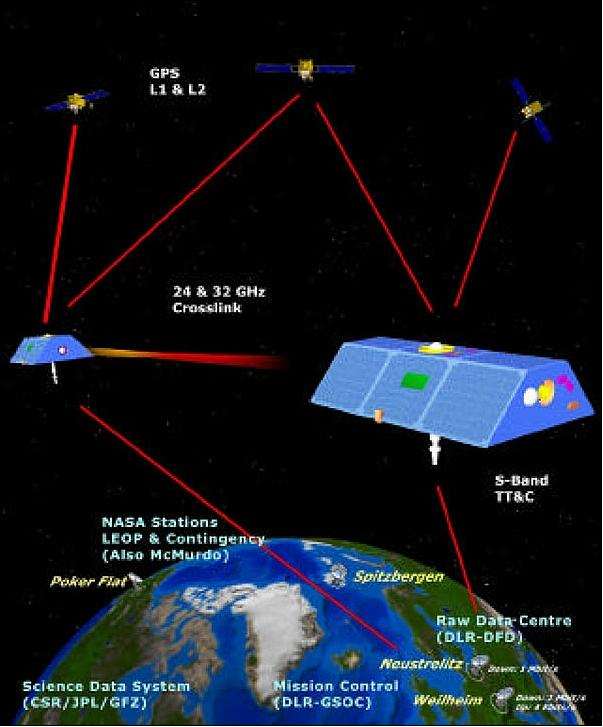
\includegraphics[width=\textwidth]{figures/GRACE_satellites.jpg}
        \end{column}
        \begin{column}{0.8\textwidth}
        \centering
        Hauteur d'eau équivalente saisonnière en mm (2002-2017) \vspace*{-1cm}
          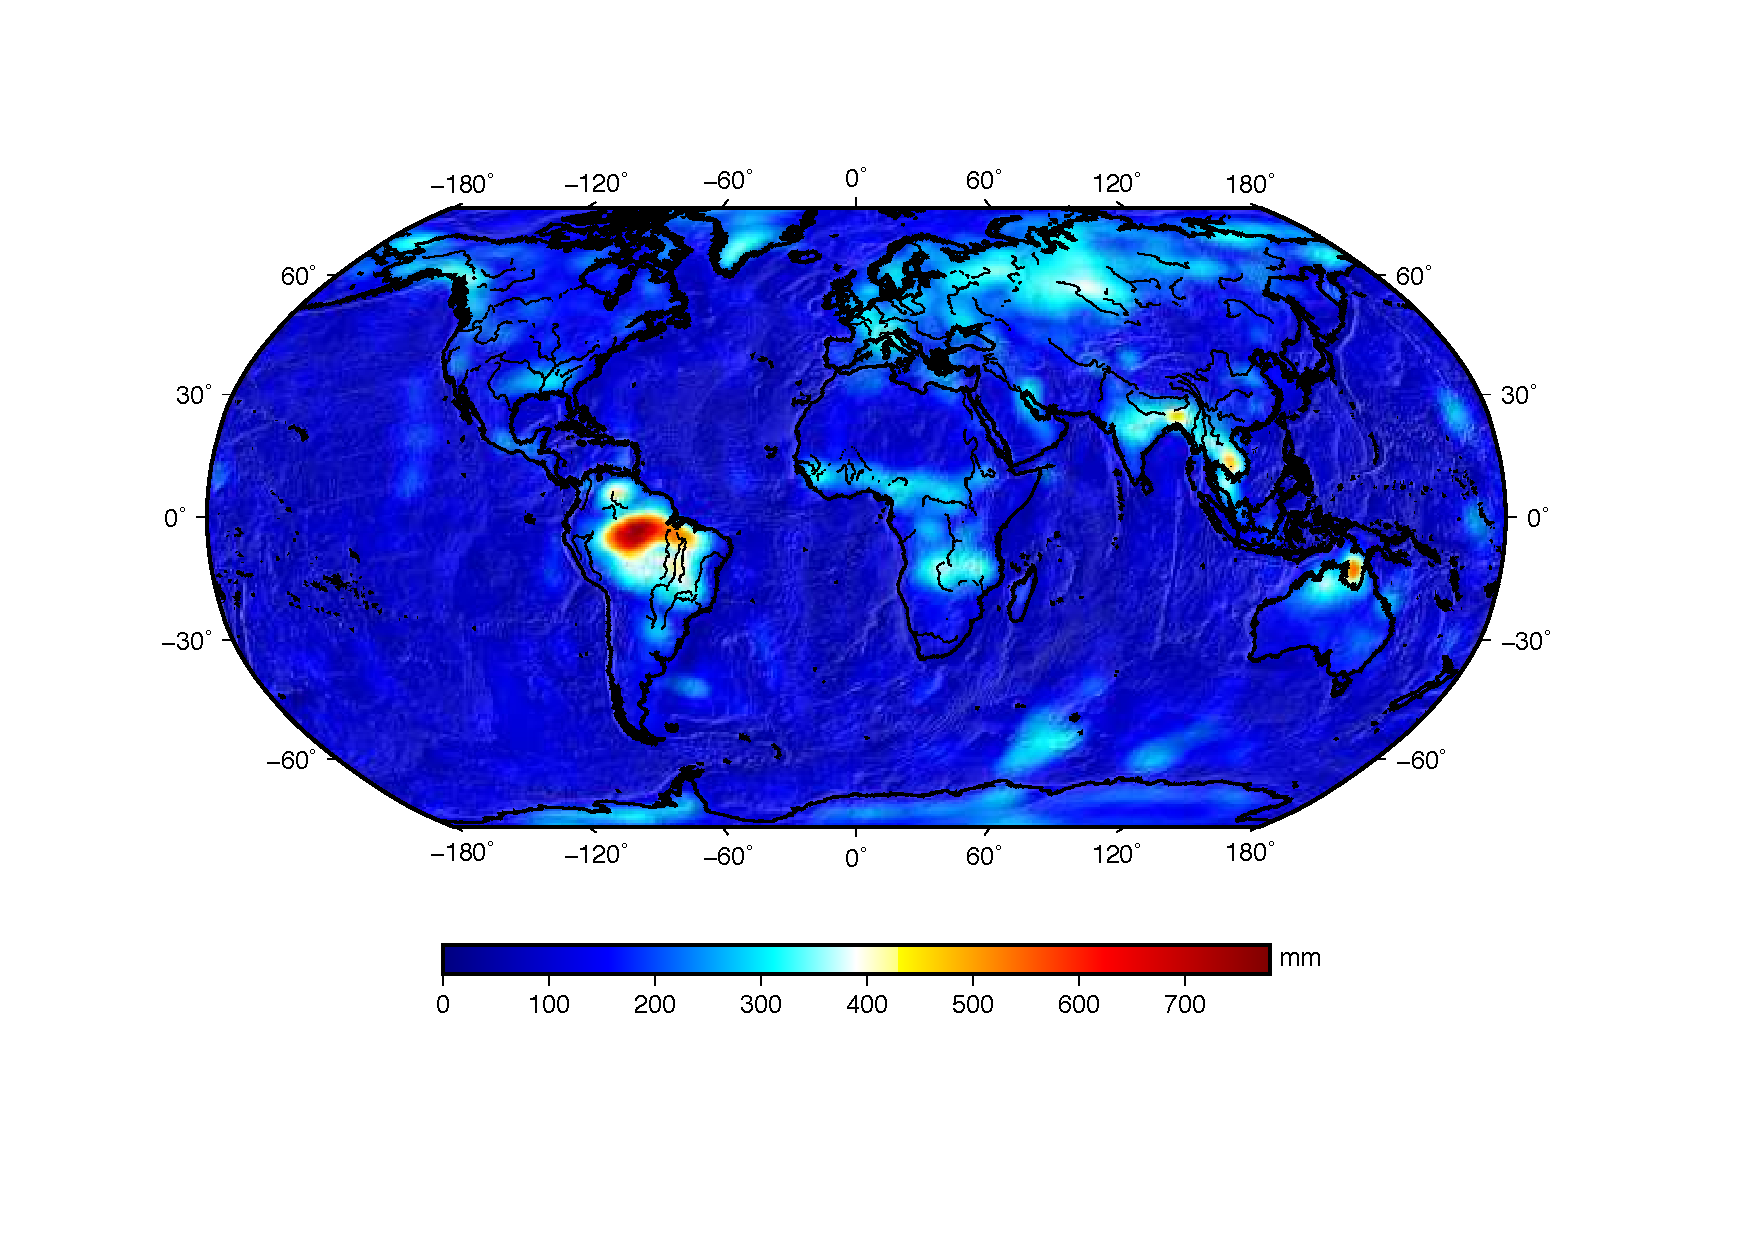
\includegraphics[width=\textwidth]{figures/global_map_grace.pdf} 
          \tiny{\textit{(Chanard et al., 2018)}}
        \end{column}
    \end{columns}
          \begin{itemize}
              \item Mission satellite tandem (2002-2017)
              \item Cartographie des variations spatio-temporelles du champ de gravité
              \item Mesure des redistributions des masses océaniques, atmosphériques et hydrologiques
              \item Résolution: $\sim$400km $\times$ 1 mois
          \end{itemize}
\end{frame}

\begin{frame}
\frametitle{Modèles environnementaux}
    \begin{columns}
        \begin{column}{0.2\textwidth}
            Hydrologiques :
            \begin{itemize}
                \item GLDAS
                \item MERRA2 Land
                \item NCEP
                \item ERA5 Land
                \item LSDM hydrology
            \end{itemize}
            Océaniques :
            \begin{itemize}
                \item ECCO
                \item NTOL
            \end{itemize}
            Atmosphériques :
            \begin{itemize}
                \item MERRA2
                \item ERA5
                \item NTAL
            \end{itemize}
        \end{column}
        \begin{column}{0.8\textwidth}
            Exemple : \textbf{GLDAS}, the Global Land Data Assimilation System\\ \\
            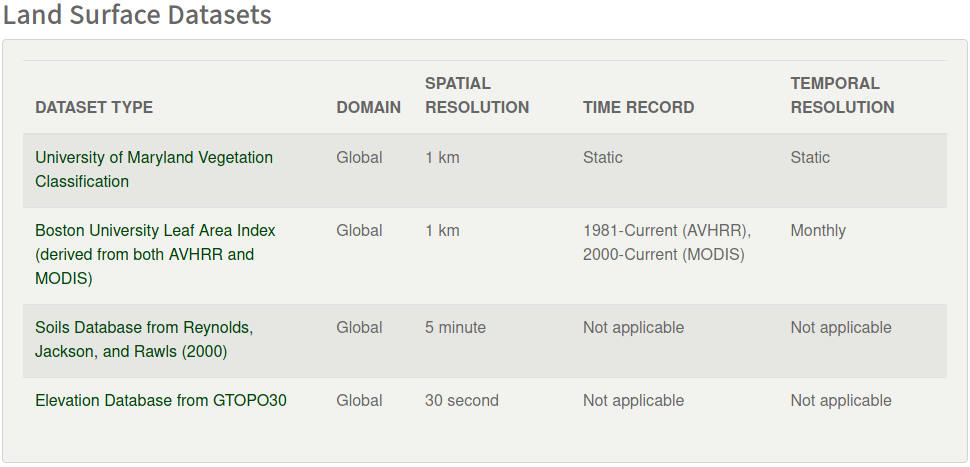
\includegraphics[width=\textwidth]{figures/obs_gldas.png}
            \begin{itemize}
              \item Plusieurs modèles physiques disponibles : NOAH, VIC, CLSM
              \item Prédiction des mouvements de masses hydrologiques
              \item Résolution: $\sim$25-100km $\times$ 3 heures
            \end{itemize}
            \begin{workblock}{}
                 \small{Travail bibliographique pour saisir le fonctionnement général des modèles de charge ci-contre.}
            \end{workblock}
        \end{column}
    \end{columns}
\end{frame}

\begin{frame}
\frametitle{Modèles environnementaux}
\centering
Exemple : \textbf{ECCO}, Estimating the Circulation and Climate of the Ocean\\
    \begin{columns}
        \begin{column}{0.5\textwidth}
            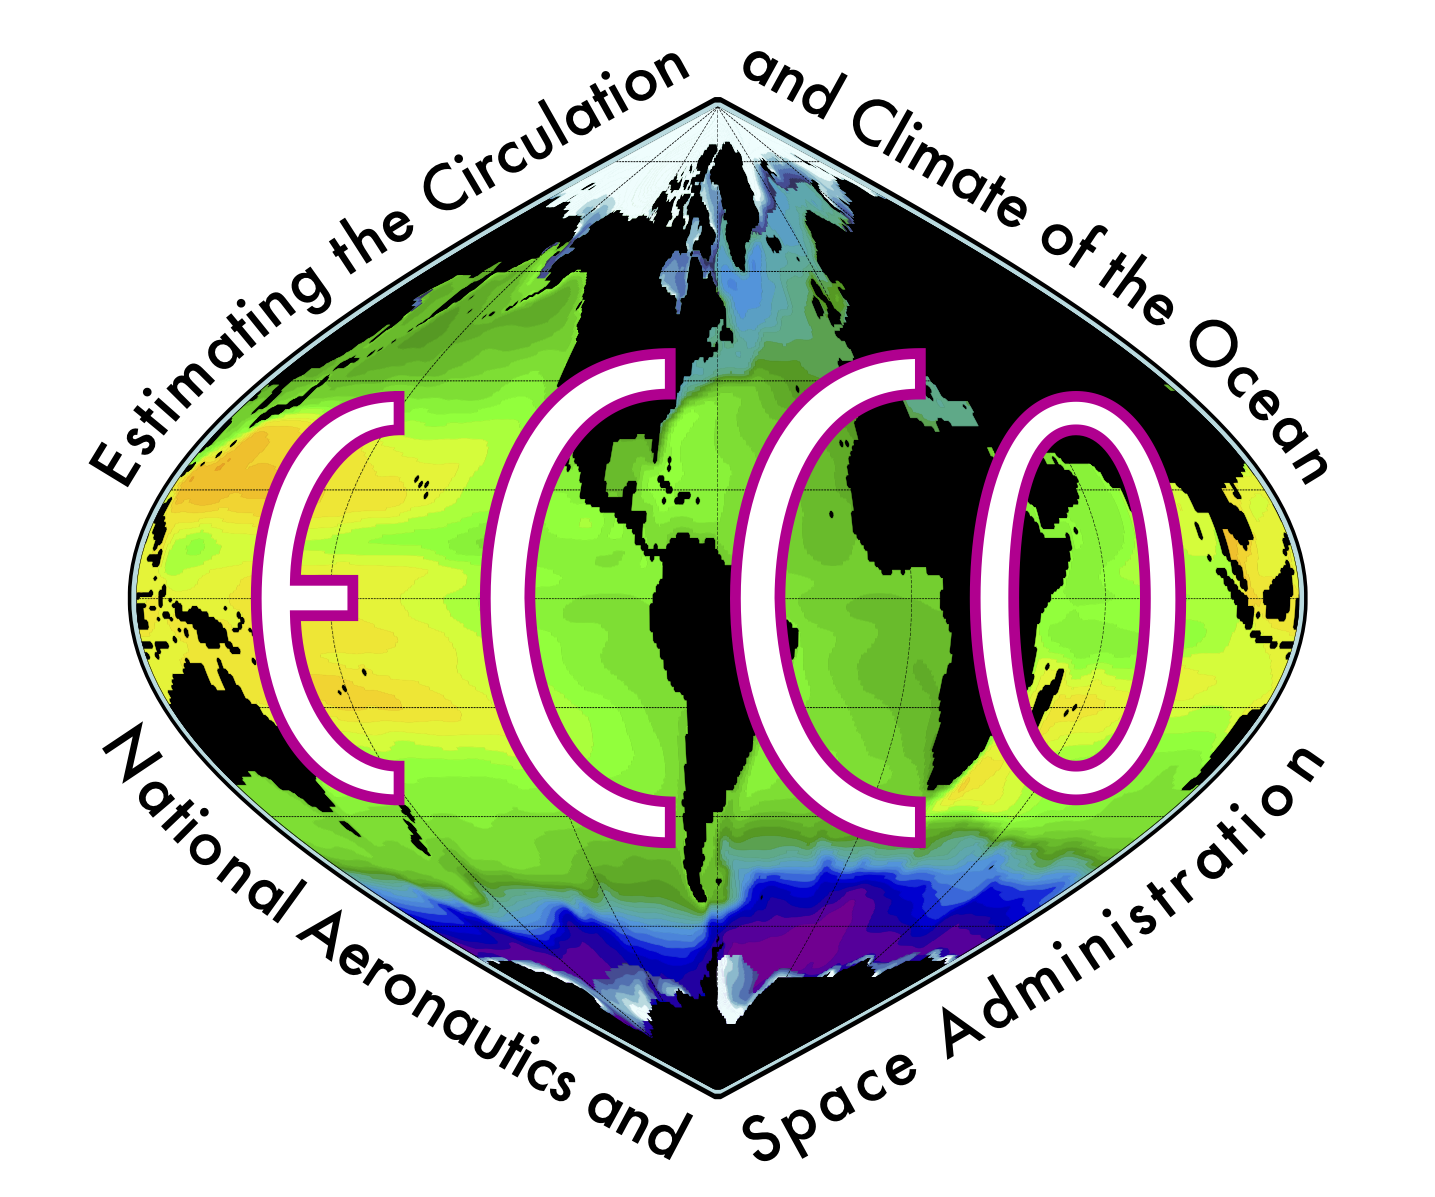
\includegraphics[width=0.7\textwidth]{figures/ecco.png}
            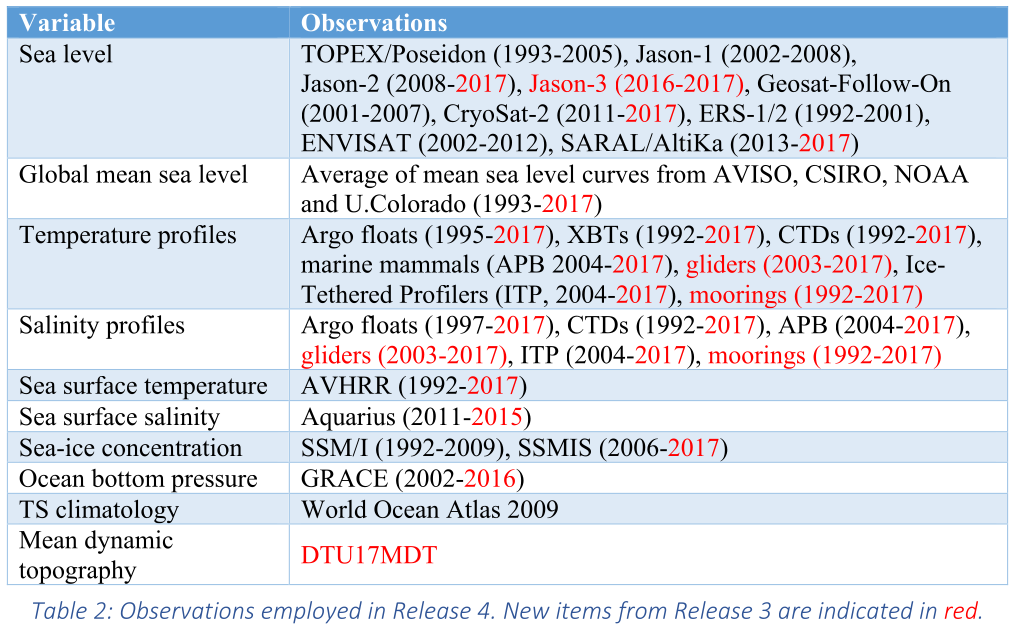
\includegraphics[width=\textwidth]{figures/obs_ecco.png}
        \end{column}
        \begin{column}{0.5\textwidth}
            \centering
            Gliders\\
            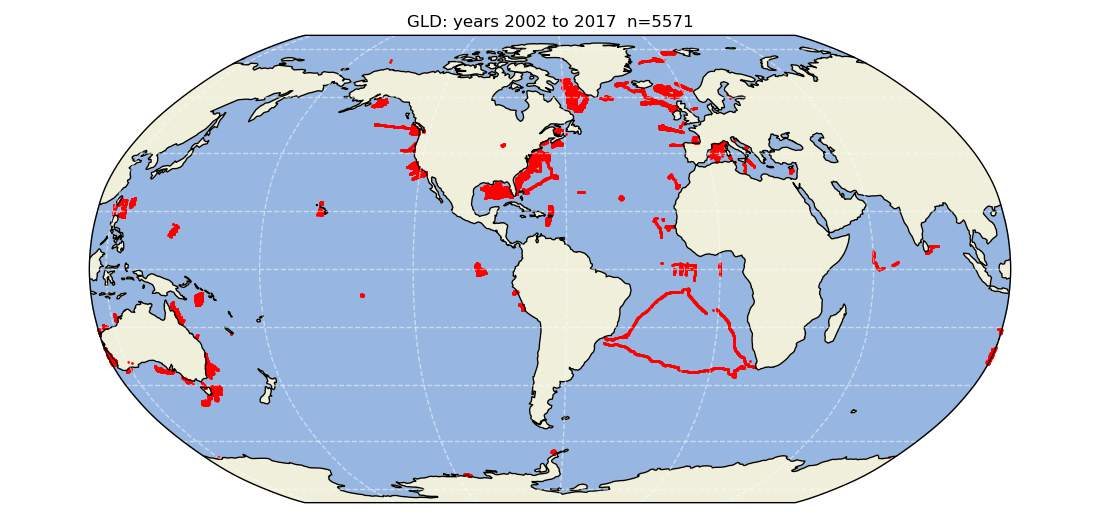
\includegraphics[width=0.7\textwidth]{figures/gliders_distribution.png} \\
            Argos\\
            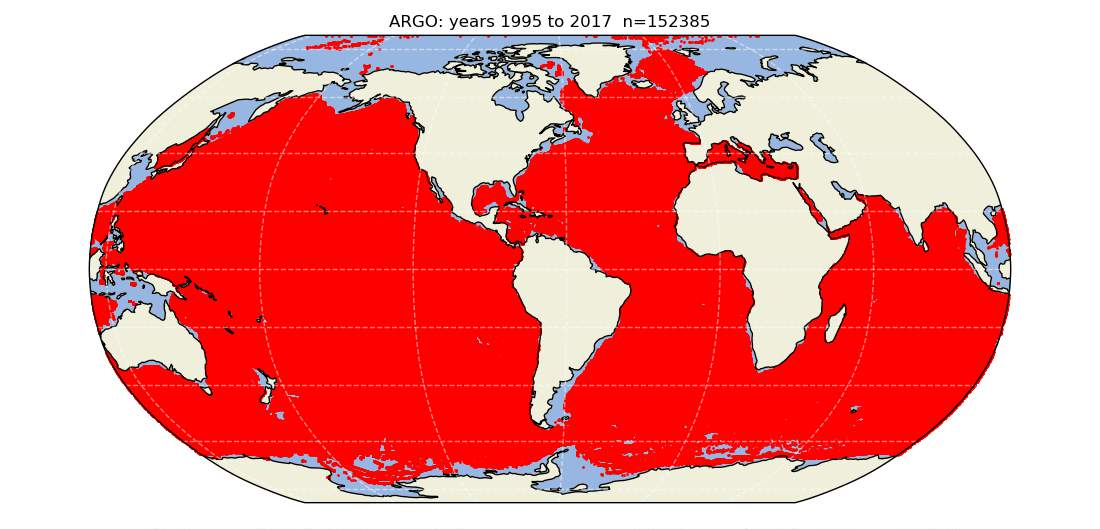
\includegraphics[width=0.7\textwidth]{figures/argos_distribution.png}
            \begin{itemize}
              \item Modèle physique : MIT general circulation model
              \item Prédiction des mouvements de masses océaniques
              \item Résolution: $\sim$100km $\times$ 1 heure/1 jour/1 mois
            \end{itemize}
            
        \end{column}
    \end{columns}
\centering
\begin{workblock}{}
     \small{Travail de conversion : Lat-Lon-Cap 90 $\rightarrow$ grille globale $\rightarrow$ coefficients en harmoniques sphériques.}
\end{workblock}
    
\end{frame}


\section[Déformations de la Terre par...]{Déformations de la Terre par des charges de surface}

\begin{frame}
\frametitle{Calcul des déformations dues aux effets de surcharge}
    \begin{columns}
    \begin{column}{0.45\textwidth}
        \centering
        \textbf{Explication physique}
        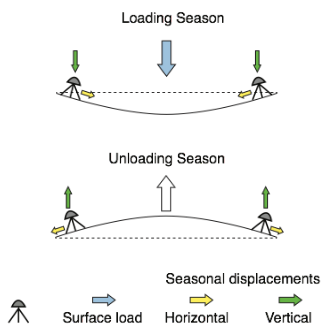
\includegraphics[width=\textwidth]{figures/schema_gps_load_vertical.png}
    \end{column}
    \begin{column}{0.37\textwidth}
    \centering
    \textbf{Modélisation}
    \small{
    \begin{equation}
    \mathcal{\sigma}(t,\phi,\lambda) = \sum_{l=1}^{\infty}\sum_{m=0}^{l} \sum_{\psi \in \{S,C\}} \sigma_{lm}^{\psi}(t)Y_{lm}^{\psi}(\phi,\lambda) \nonumber
    \end{equation}
    }
        \small{
        \begin{align}
        dE(t,\phi,\lambda) &= \frac{4\pi R_E^3}{M_E}\sum_{l=0}^{\infty}\sum_{m=0}^{l} \sum_{\psi \in \{S,C\}} \color{blue} \frac{ \mathscr{l}_l}{2l+1}  \color{green}\sigma_{lm}^{\psi}(t)\color{black}\frac{1}{\cos \phi} \frac{\partial Y_{lm}^{\psi}}{\partial \lambda}(\phi,\lambda) \nonumber\\
        dN(t,\phi,\lambda) &= \frac{4\pi R_E^3}{M_E}\sum_{l=0}^{\infty}\sum_{m=0}^{l} \sum_{\psi \in \{S,C\}} \color{blue}\frac{ \mathscr{l}_l}{2l+1} \color{green}\sigma_{lm}^{\psi}(t) \color{black} \frac{\partial Y_{lm}^{\psi}}{\partial \phi}(\phi,\lambda) \label{def} \nonumber\\
        dU(t,\phi,\lambda) &= \frac{4\pi R_E^3}{M_E}\sum_{l=0}^{\infty}\sum_{m=0}^{l} \sum_{\psi \in \{S,C\}} \color{blue}\frac{\mathscr{h}_l}{2l+1} \color{green} \sigma_{lm}^{\psi}(t) \color{black} Y_{lm}^{\psi}(\phi,\lambda) \nonumber
        \end{align}
        }
    \end{column}
    
\end{columns}

\begin{workblock}{}
\begin{columns}
        \begin{column}{0.09\textwidth}
        \centering
        
\includegraphics[ width=\textwidth]{figures/ALIEDOCS_logo.png}
        \end{column}
        \begin{column}{0.89\textwidth}
         \small{Amélioration du service de calcul de déformation ALIEDOCS initié en projet développement de 2ème année.}
        \end{column}
\end{columns}


\end{workblock}
\end{frame}

\begin{frame}
\frametitle{Prédiction d'un modèle à une station}
\begin{columns}
        \begin{column}{0.6\textwidth}

            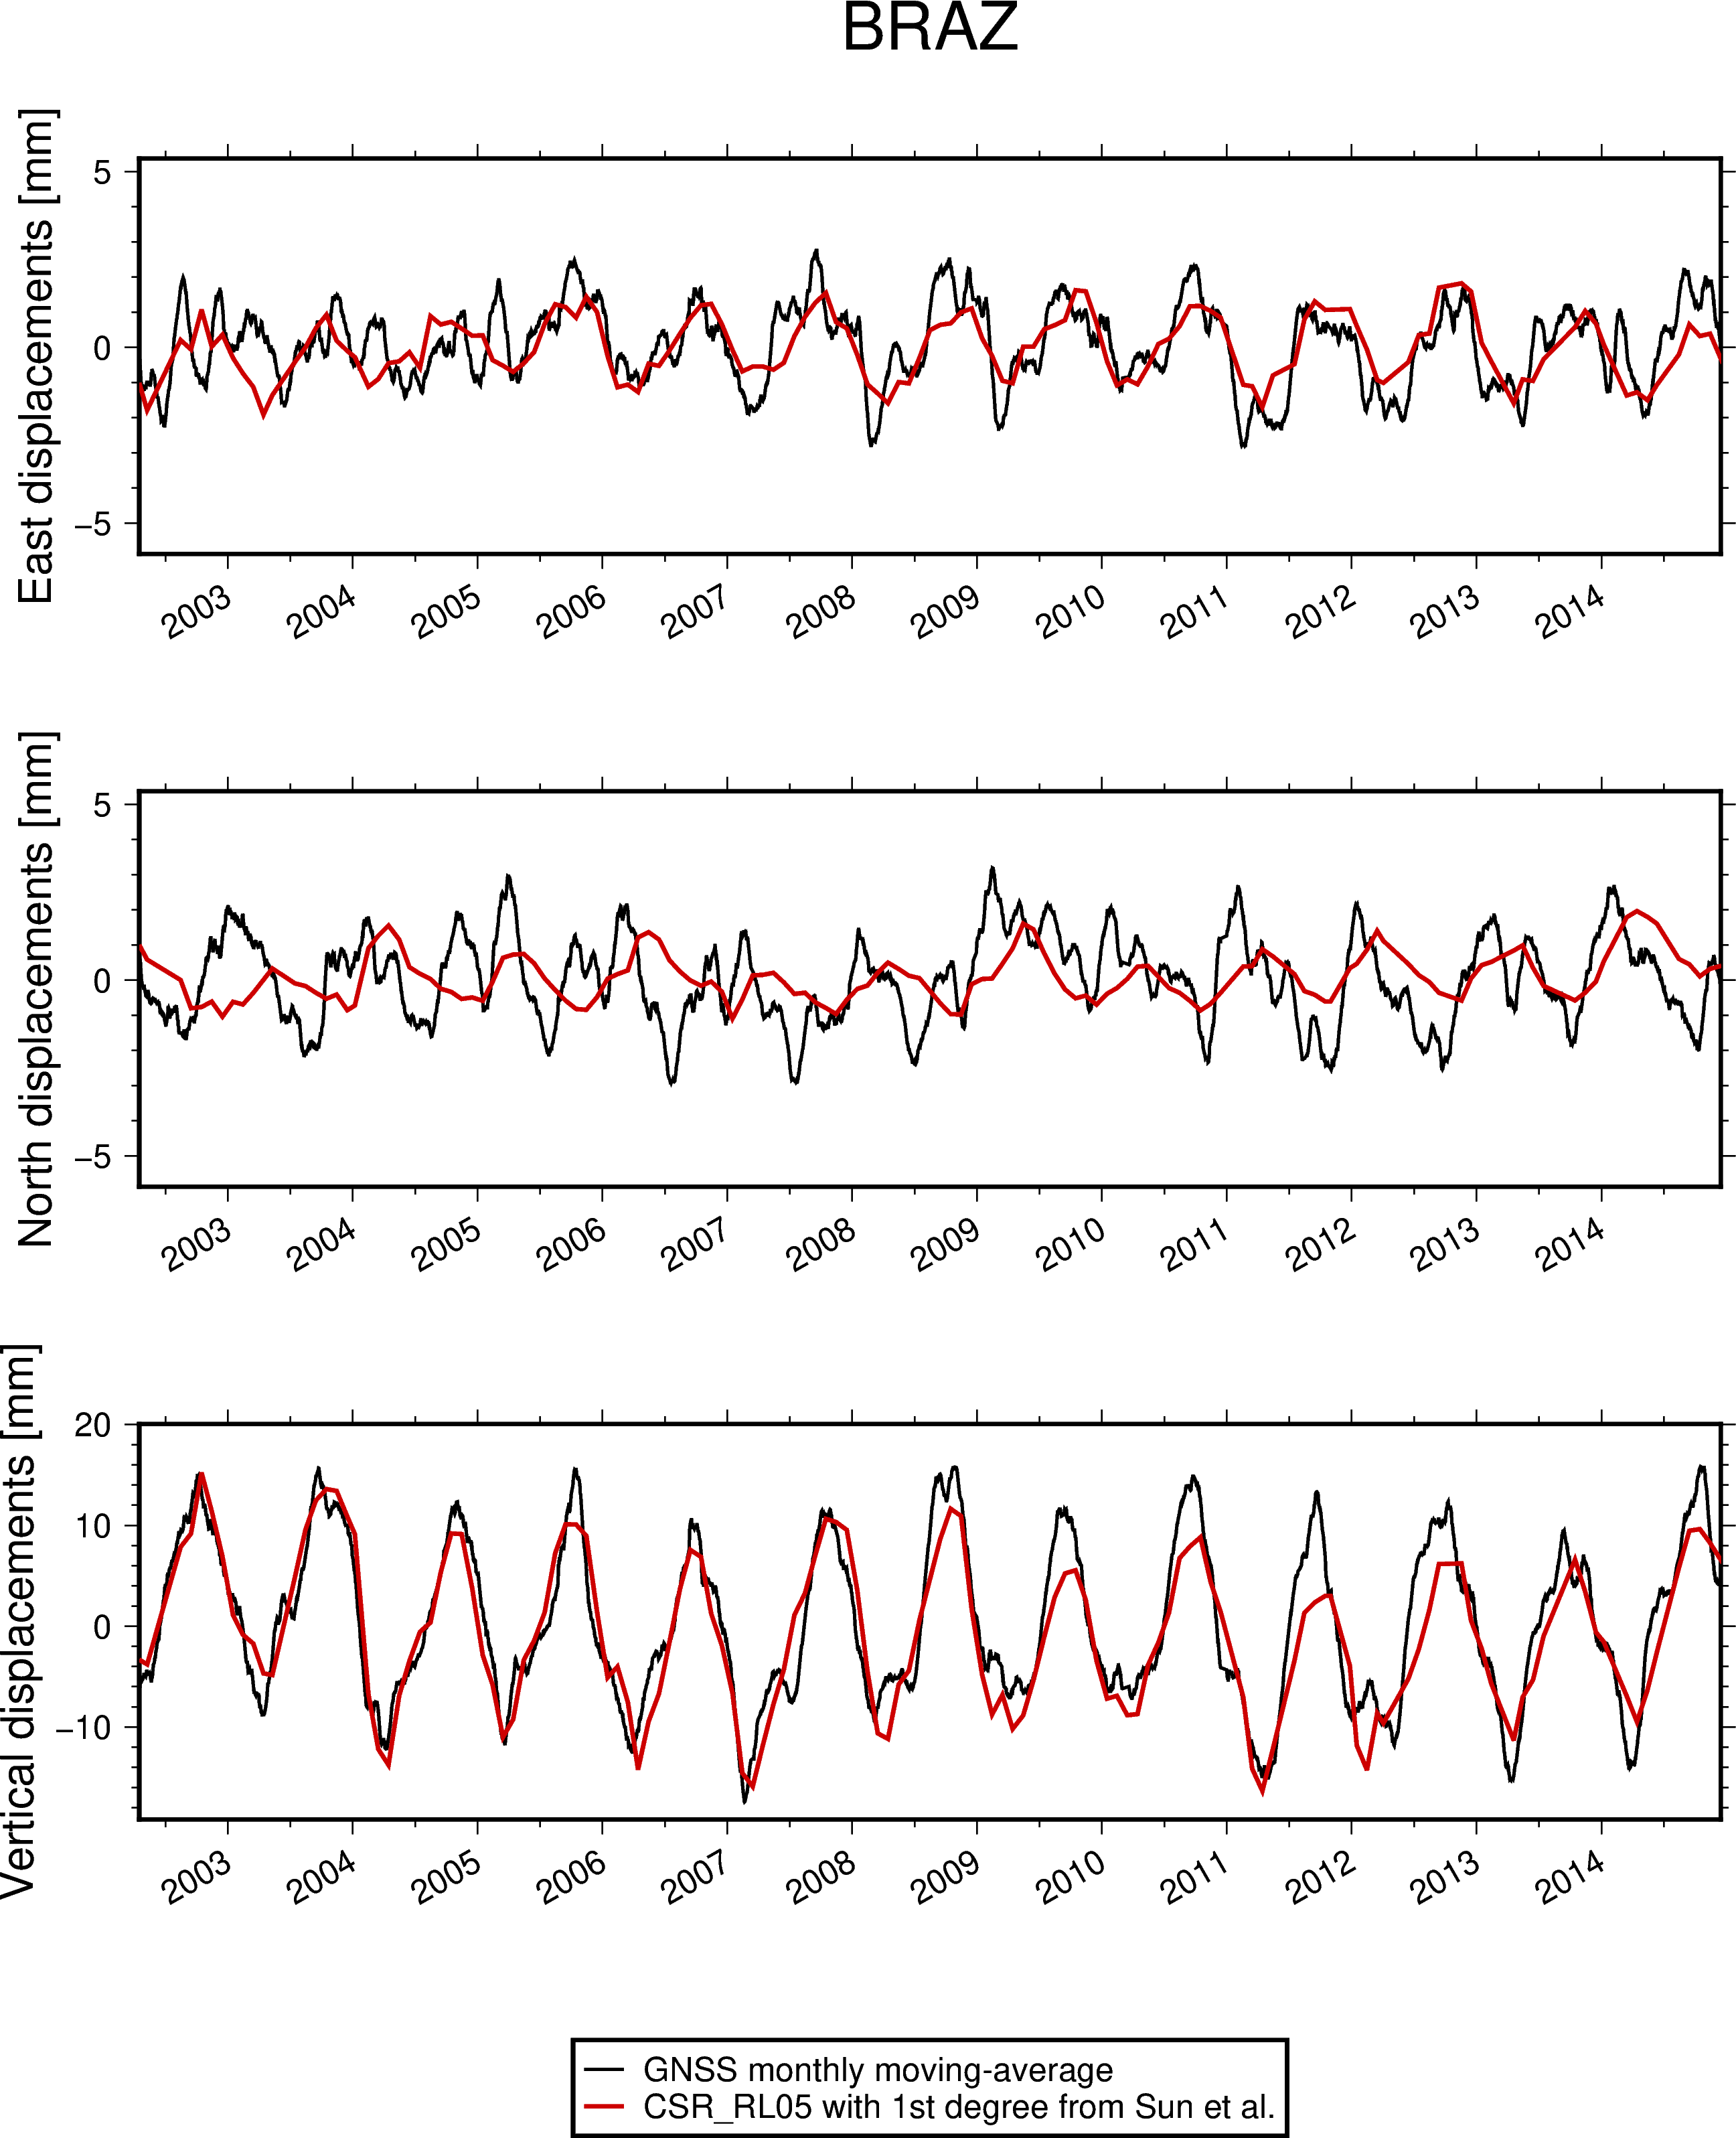
\includegraphics[width=\textwidth]{figures/BRAZ_GRACE_CSR5_w1dSun_vs_IG2.png}
        \end{column}
        \begin{column}{0.45\textwidth}
            \begin{itemize}
                \item Utilisation du degré-1 estimé par Sun et al. (2016) \\(degré-1 non mesuré par GRACE)
                \item Insuffisante sur les composantes planimétriques également vraie sur l'ensemble du réseau
            \end{itemize}   
        \end{column}
\end{columns}


\end{frame}

%\begin{frame}
%\frametitle{Comparaison de modèles}
%Carte de réduction de variance du signal complet (sans séparation annuel/semi-annuel)
%\begin{workblock}{}
% \small{Analyse statistique GNSS-modèles}
%\end{workblock}
%\end{frame}


\section[Particularité des charges de...]{Particularité des charges de très grande longueur d'onde}

\begin{frame}
\frametitle{Charges de grandes longueurs d'onde : degré-1}
\begin{columns}
        \begin{column}{0.5\textwidth}
            \begin{itemize}
                \item Peut s'obtenir par inversion d'un réseau de stations GNSS (après retrait des charges de degré 2 et supérieurs d'un modèle)
                \item la figure ci-contre montre que le degré-1 inversé à partir du réseau IGS et de différentes solutions GRACE apporte une meilleure prédiction du signal GNSS pour les composantes Nord et Est. 
            \end{itemize}
        \end{column}
        \begin{column}{0.5\textwidth}
            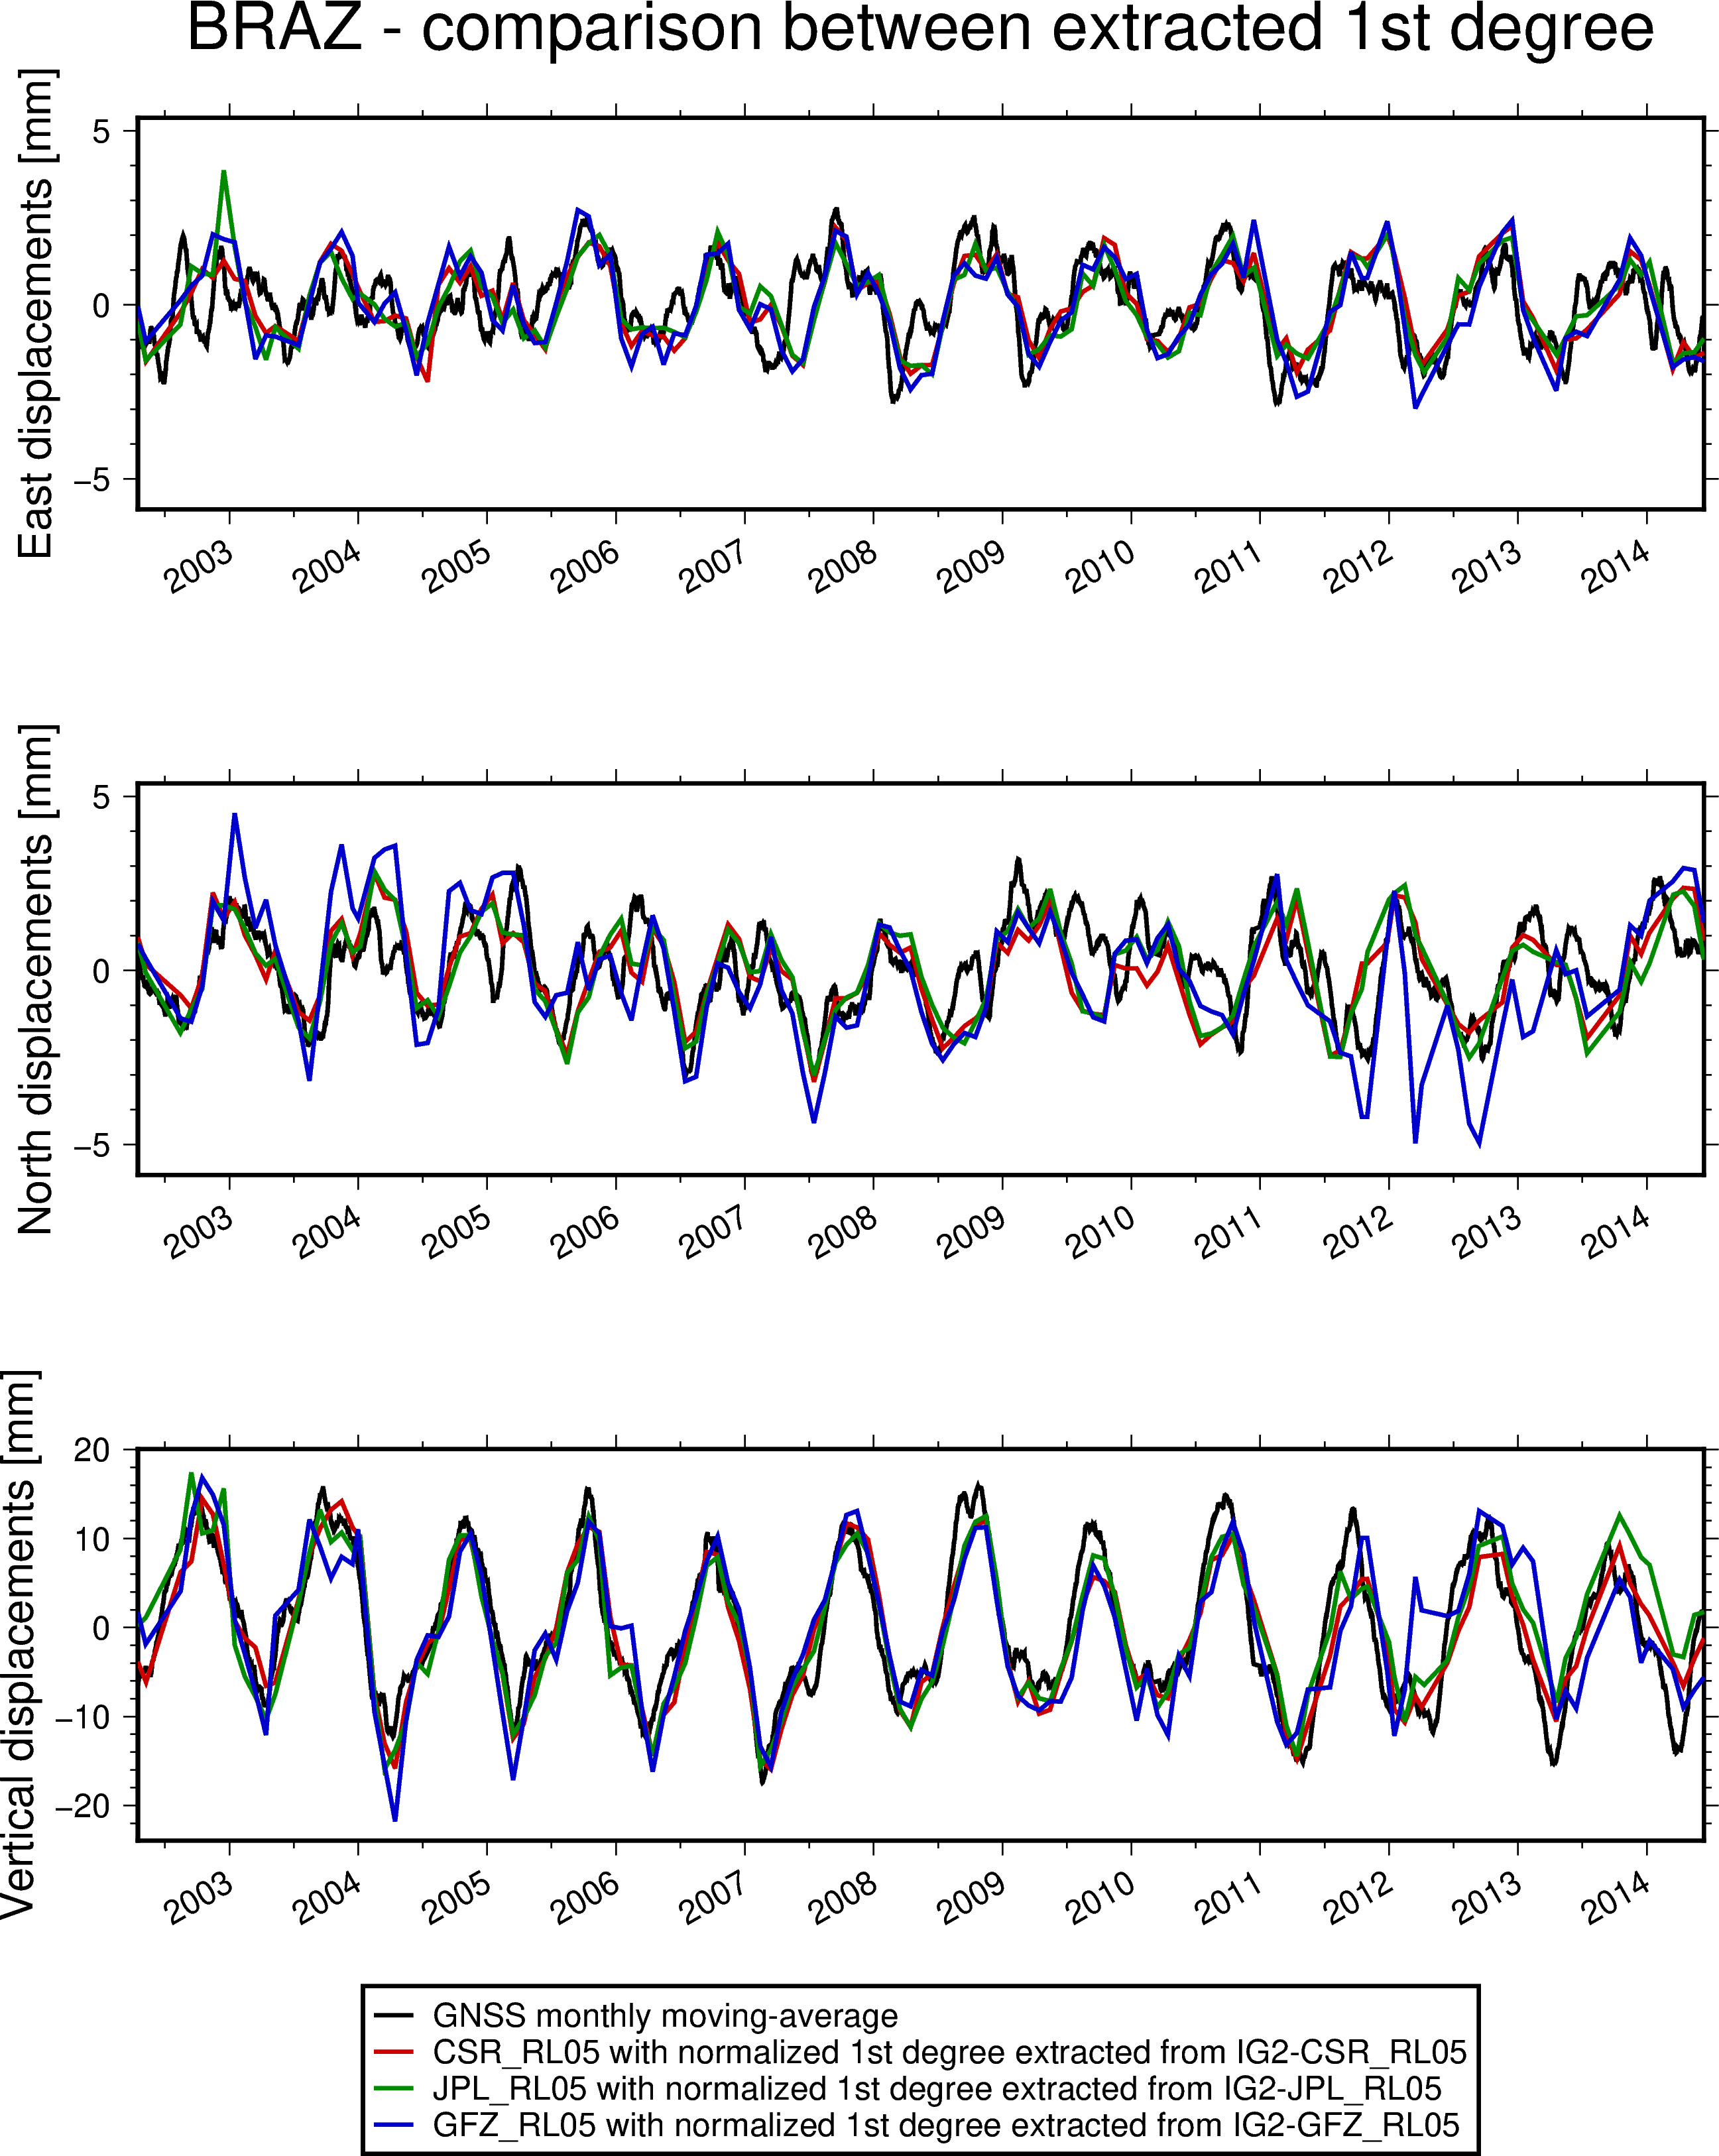
\includegraphics[width=\textwidth]{figures/BRAZ_w1d_from_inversion.png}
        \end{column}
\end{columns}

\begin{workblock}{}
 \small{Développement d'un module Python pour le calcul d'inversion et la manipulation du degré-1 sous différents formats}
\end{workblock}
\end{frame}

\begin{frame}
\frametitle{Mouvement du géocentre}
    \centering
    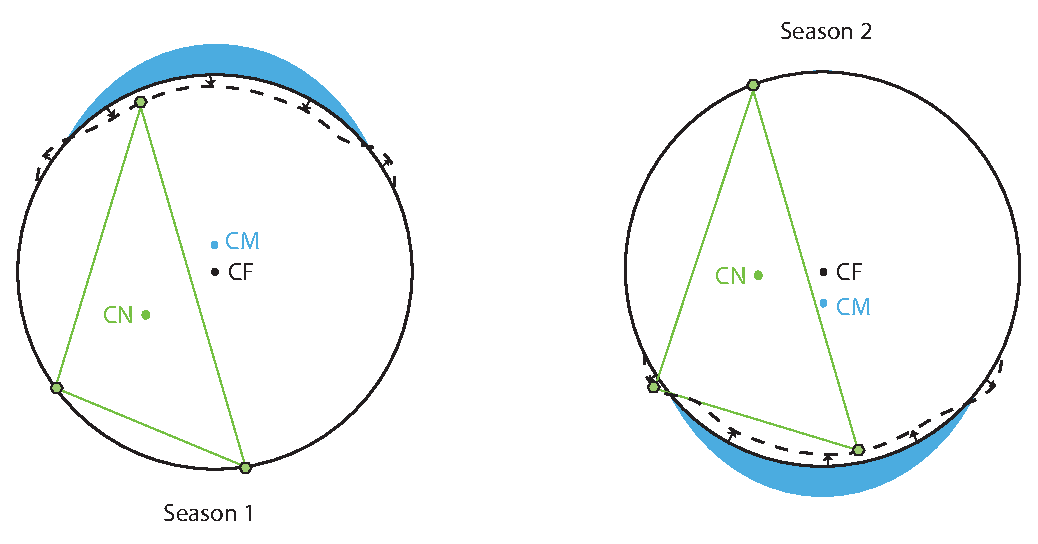
\includegraphics[height=0.40\textheight]{figures/scheme_geocenter.eps}
    \begin{itemize}
        \item Le mouvement du géocentre désigne le déplacement relatif entre le centre de masses (CM) du système Terre et celui du centre de figure (CF)
        \item Le centre de réseau (CN) correspond au centre géométrique de toutes les stations d'un réseau. C'est celui que l'on obtient par inversion d'un réseau.
        \item On fait l'hypothèse que les charges de degré-1 représentent le mouvement du géocentre.
    \end{itemize}
    
    \begin{equation}
        \Delta r_{{{\text{CF}} - {\text{CM}}}} = \sqrt 3 \left( {\frac{{\left[ {h_{1}^{'} } \right]_{CE} + 2\left[ {l_{1}^{'} } \right]_{CE} }}{3} - 1} \right)\frac{{\rho_{\text{S}} }}{{\rho_{\text{E}} }}
        \vec{\sigma_1} \nonumber
    \end{equation}
    où $\vec{\sigma_1}=(\sigma_{11}^{C}, \sigma_{11}^{S}, \sigma_{10})$

\end{frame}

\begin{frame}
\frametitle{Comparaison du mouvement du géocentre}
\begin{columns}
        \begin{column}{0.6\textwidth}
             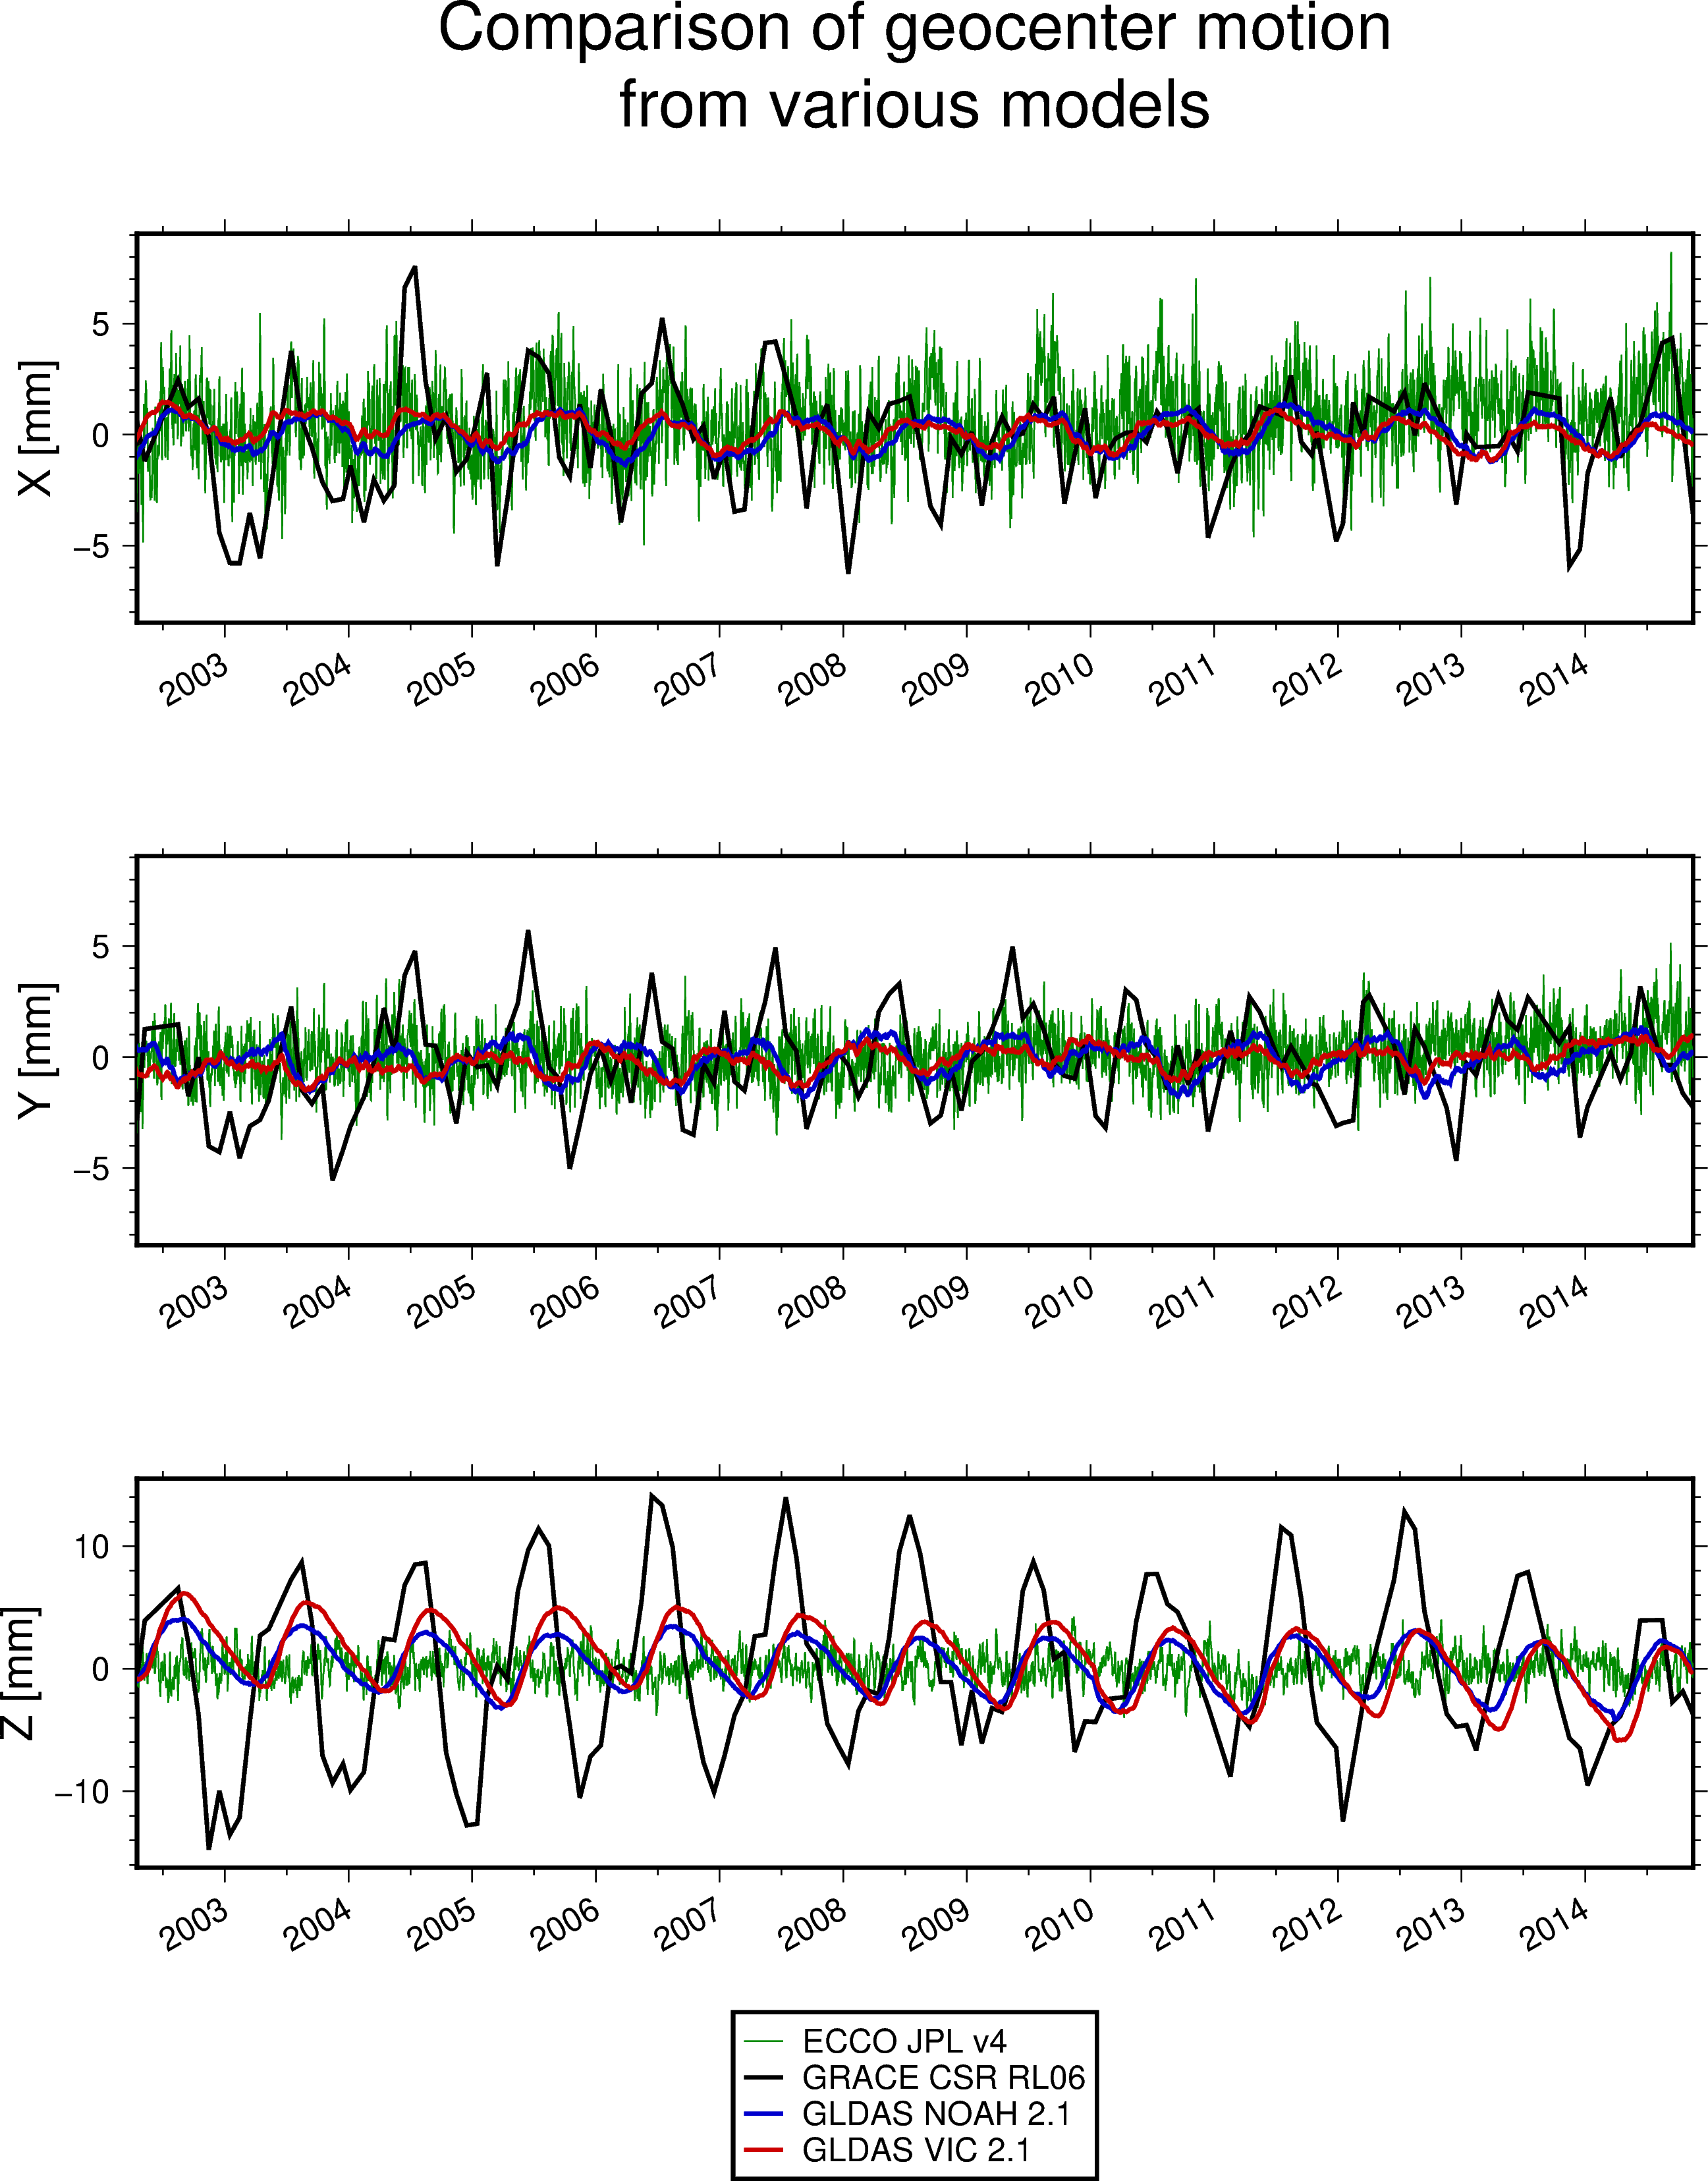
\includegraphics[height=0.8\textheight]{figures/comparison_geocenter_motion.png}   
        \end{column}
        \begin{column}{0.4\textwidth}
            Le mouvement prédit par inversion du degré-1 à partir d'un réseau GNSS présente une amplitude bien plus importante que les modèles de charge et un léger décalage de phase. Ainsi, deux hypothèses :
\begin{itemize}
    \item Les modèles de charge ne prédisent pas toute la charge effective
    \item le signal GNSS contient autre chose que les déformations dues aux effets de charge
\end{itemize}
        \end{column}
\end{columns}



\end{frame}


\section*{Conclusion}

\begin{frame}
\frametitle{Conclusion}
\begin{block}{Conclusion}
     \begin{itemize}
        \item Préparation et normalisation de nombreux modèles de charge pour le calcul de déformations via ALIEDOCS.
        \item Étude et inversion du degré-1 à partir d'un réseau GNSS et d'un modèle de charges.
        \item Analyse statistique comparée des différents modèles de charges (à suivre...).
\end{itemize}
     \end{block}

\begin{block}{Perspectives}
\begin{itemize}
    \item Expliquer le reste du signal par la déformation thermoélastique du sol et/ou du monument GNSS.
\end{itemize}
\begin{columns}
        \begin{column}{0.6\textwidth}
            \centering
            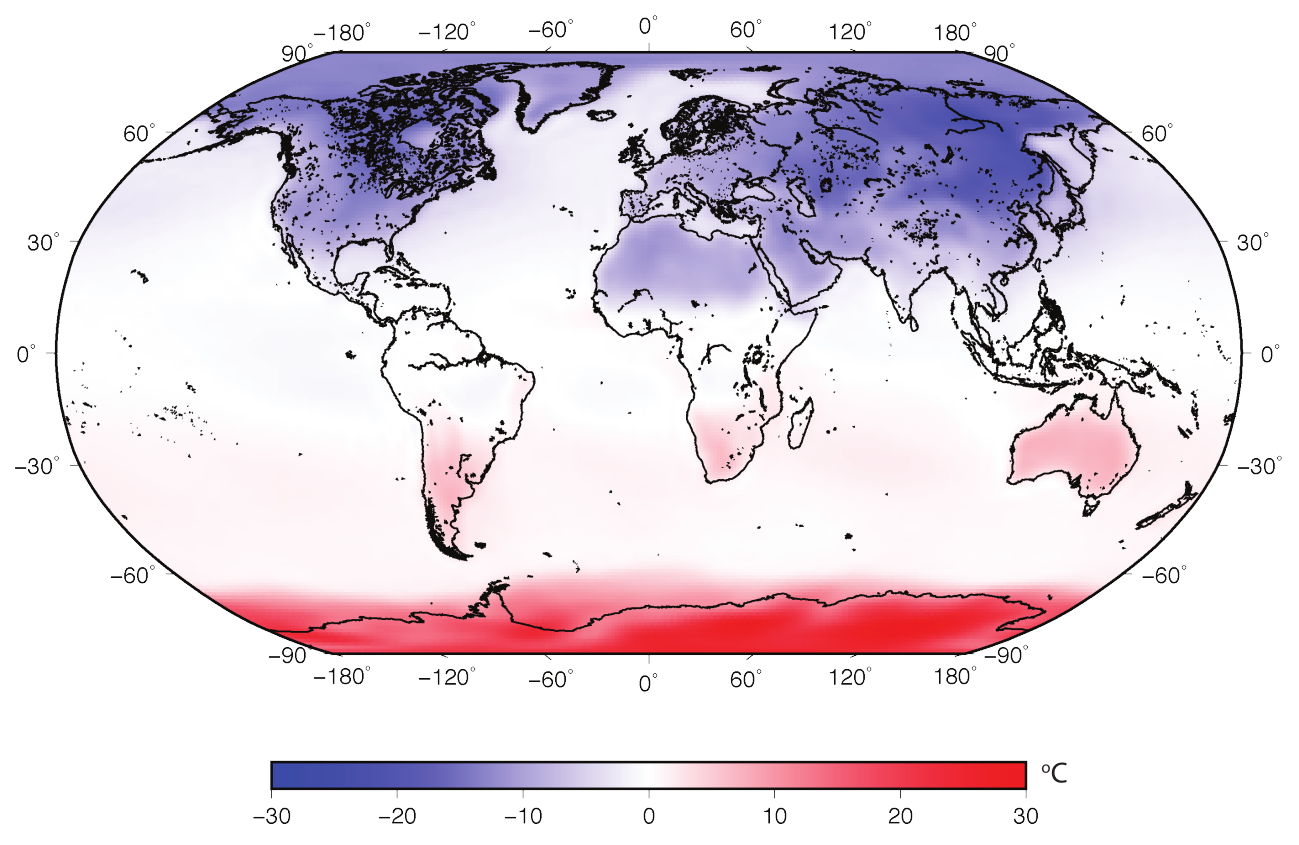
\includegraphics[height=0.26\textheight]{figures/temperature_field.png}
        \end{column}
        \begin{column}{0.4\textwidth}
            \small{Température moyenne en Janvier comparée à la température moyenne annuelle sur la période 2002-2015}
        \end{column}
\end{columns}
\begin{itemize}
    \item Étudier la variabilité de l'inversion du degré-1 en fonction de l'homogénéité du réseau utilisé.
\end{itemize}


\end{block}
\end{frame}

\end{document}

% Travail accompli à mentionner:
% - Amélioration du serveur de calcul (résolution de bugs, optimisation du calcul)
% - Développement d'une librairie Python pour l'inversion du degré-1
% - Développement d'une librairie Python pour extraire les signaux annuels/semi-annuels.
% - Travail bibliographique sur les modèles
